\section{26 Oct 2023 - Activity: 1-Dimensional Travelling
Waves}\label{oct-2023---activity-1-dimensional-travelling-waves}

\href{https://en.wikipedia.org/wiki/Wave_equation}{Wave equations} are
common to all branches of physics. In fact, many modern research topics
include some investigations that use wave theory. So useful is the
concept of a wave, that we adapted it for quantum mechanics in the form
of the
\href{https://en.wikipedia.org/wiki/Schr\%C3\%B6dinger_equation}{Schrodinger
Equation} and the position representation of the wavefunction
(\(\psi(x,t)\)). While wildly useful and broadly applicable, we need to
build up some intuition and use cases for waves. We will start with the
1D wave equation:

\[\dfrac{\partial^2 f(z,t)}{dz^2} = \dfrac{1}{v^2}\dfrac{\partial^2 f(z,t)}{dt^2}\]

As we discussed, any function of the form:

\[f(z,t) = g(z+vt)+h(z-vt)\]

solves the 1D wave equation. One way to think about this what this
solution is showing is that some smooth function \(g(z)\) and another
smooth function \(h(z)\) individually solve the wave equation if they
just move to the left for \(g\) and to the right for \(f\). Furthermore
because this PDE is linear (containing only linear derivatives of \(z\)
and \(t\), i.e., no squares or functions of them),
\href{https://en.wikipedia.org/wiki/Superposition_principle}{superposition}
holds. And we can simply add solutions together linearly to get new
solutions!

\subsection{Travelling Wave Solutions}\label{travelling-wave-solutions}

That is all well and good, but we need a common language. A grammar to
understand our solutions. These are basis functions, they are the things
we all agree on that describe the ``space'' of the solutions. You have
seen these already in our study of normal modes. Our sinusoidal
solutions, the frequencies and amplitudes of the modes themselves,
provide a set of basis functions that can describe the general motion of
the coupled SHOs. What's nice about that choice is that we can reproduce
it because we all agree to solve the same eigenvalue problem.

For the 1D wave equation, these functions are
\href{https://en.wikipedia.org/wiki/Periodic_travelling_wave}{Travelling
Wave Solutions}. The describe the simplest motion of a travelling wave:
single frequency oscillation over an infinite domain. There's no end
points to worry about, and only one frequency. Also, it just moves to
the left or to the right. You can probably see how multiple dimensions
result in much more complexity. A basic traveling wave solution is:

\[f(z,t) = A cos(kz-\omega t+\phi)\]

You can show that this equation satisfies the wave equation with
\(v=\omega/k\).

More importantly, does a linear sum do so?

\textbf{✅ Do this}

Demonstrate that this proposed general solution:

\[F(z,t) = \sum_i^n A_i\:cos(k_i z - \omega t + \phi_i)\]

solves the wave equation.

\subsection{Looking at Travelling Wave
Solutions}\label{looking-at-travelling-wave-solutions}

Let's investigate several scenarios for travelling wave solutions:

\begin{enumerate}
\def\labelenumi{\arabic{enumi}.}
\tightlist
\item
  A single travelling wave (done for you with different representations)
\item
  The superposition of two waves (not close frequencies; close
  amplitudes)
\item
  The superposition of two waves (close frequencies; close amplitudes)
\item
  The superposition of two waves (not close frequencies; not close
  amplitudes)
\item
  The superposition of two waves (close frequencies; not close
  amplitudes)
\item
  The superposition of three waves (make adjustments to test your
  intuition from two waves)
\end{enumerate}

Make your choices, but also vary them a bit. You can investigate things
like widgets (e.g.,
\href{https://matplotlib.org/stable/gallery/widgets/slider_demo.html}{sliders})
which make this stuff more interactive, but regular plots are totally
fine.

\textbf{✅ Do this}

Here is my suggestion and a challenge:

\begin{enumerate}
\def\labelenumi{\arabic{enumi}.}
\tightlist
\item
  Plot your solutions in 2D for a fixed location (e.g., \(x=0\)) for all
  time (\(f\) vs \(t\))
\item
  Plot your solutions in 2D for a given time (e.g., \(t=0\)) for all x
  (\(f\) vs \(x\))
\item
  Plot your solutions in 3D using the \(x-y\) plane as positions vs time
  and using \(z\) for \(f\) (what does this representation buy you? Is
  it more or less useful than the above two?)
\item
  Challenge (animate your plots). Matplotlib can use the animation api.
  \href{https://matplotlib.org/2.0.2/examples/animation/simple_anim.html}{Here's
  a simple script}.
\end{enumerate}

\begin{Shaded}
\begin{Highlighting}[]
\ImportTok{import}\NormalTok{ numpy }\ImportTok{as}\NormalTok{ np}
\ImportTok{import}\NormalTok{ matplotlib.pyplot }\ImportTok{as}\NormalTok{ plt}
\ImportTok{from}\NormalTok{ mpl\_toolkits.mplot3d }\ImportTok{import}\NormalTok{ Axes3D}
\ImportTok{from}\NormalTok{ matplotlib.animation }\ImportTok{import}\NormalTok{ FuncAnimation}
\ImportTok{from}\NormalTok{ IPython.display }\ImportTok{import}\NormalTok{ HTML}
\OperatorTok{\%}\NormalTok{matplotlib inline}

\end{Highlighting}
\end{Shaded}

\subsubsection{Single Travelling Wave}\label{single-travelling-wave}

Here's the plots for a single travelling wave with \(A=1\),
\(\lambda = 2\), \(\omega=2\pi\), and \(\phi=0\).

\[f(z,t) = A cos(kz-\omega t+\phi)\]

First we will create the wave. This is a little bit difficult because
both \(x\) and \(t\) can vary, but we've made functions of two
dimensions before using `\texttt{meshgrid}, so we can just employ that
with a little function to complete the wave.

\begin{Shaded}
\begin{Highlighting}[]
\CommentTok{\# Parameters}
\NormalTok{A }\OperatorTok{=} \FloatTok{1.0}           \CommentTok{\# Amplitude}
\NormalTok{lambda\_ }\OperatorTok{=} \FloatTok{2.0}     \CommentTok{\# Wavelength (underscore needed because lambda is a reserved word)}
\NormalTok{f }\OperatorTok{=} \FloatTok{1.0}           \CommentTok{\# Frequency in Hz}
\NormalTok{phi }\OperatorTok{=} \FloatTok{0.0}         \CommentTok{\# Phase constant in radians}

\NormalTok{k }\OperatorTok{=} \DecValTok{2} \OperatorTok{*}\NormalTok{ np.pi }\OperatorTok{/}\NormalTok{ lambda\_}
\NormalTok{omega }\OperatorTok{=} \DecValTok{2} \OperatorTok{*}\NormalTok{ np.pi }\OperatorTok{*}\NormalTok{ f}

\CommentTok{\# Define the wave equation}
\KeywordTok{def}\NormalTok{ wave(x, t):}
    \ControlFlowTok{return}\NormalTok{ A }\OperatorTok{*}\NormalTok{ np.sin(k }\OperatorTok{*}\NormalTok{ x }\OperatorTok{{-}}\NormalTok{ omega }\OperatorTok{*}\NormalTok{ t }\OperatorTok{+}\NormalTok{ phi)}

\CommentTok{\# Generate x and t values}
\NormalTok{x }\OperatorTok{=}\NormalTok{ np.linspace(}\DecValTok{0}\NormalTok{, }\DecValTok{4} \OperatorTok{*}\NormalTok{ lambda\_, }\DecValTok{100}\NormalTok{)}
\NormalTok{t }\OperatorTok{=}\NormalTok{ np.linspace(}\DecValTok{0}\NormalTok{, }\DecValTok{2}\OperatorTok{/}\NormalTok{f, }\DecValTok{100}\NormalTok{)}

\NormalTok{X, T }\OperatorTok{=}\NormalTok{ np.meshgrid(x, t)  }\CommentTok{\# Create a meshgrid for x and t values}
\NormalTok{Y }\OperatorTok{=}\NormalTok{ wave(X, T)  }\CommentTok{\# Compute the amplitude for every combination of x and t}
\end{Highlighting}
\end{Shaded}

\paragraph{Plotting amplitide vs
location}\label{plotting-amplitide-vs-location}

Every location is waving, so here we look at all location at a single
time. And then we plot the amplitude of the wave at that location. We
can do this for different times.

\begin{Shaded}
\begin{Highlighting}[]
\CommentTok{\# Plot amplitude vs. position for different times}
\NormalTok{times\_to\_plot }\OperatorTok{=}\NormalTok{ [}\DecValTok{0}\NormalTok{, }\FloatTok{0.25}\OperatorTok{/}\NormalTok{f, }\FloatTok{0.5}\OperatorTok{/}\NormalTok{f, }\FloatTok{0.75}\OperatorTok{/}\NormalTok{f]  }\CommentTok{\# Chosen specific times to show one complete cycle}

\NormalTok{plt.figure(figsize}\OperatorTok{=}\NormalTok{(}\DecValTok{10}\NormalTok{, }\DecValTok{6}\NormalTok{))}

\ControlFlowTok{for}\NormalTok{ plot\_time }\KeywordTok{in}\NormalTok{ times\_to\_plot:}
\NormalTok{    plt.plot(x, wave(x, plot\_time), label}\OperatorTok{=}\SpecialStringTok{f\textquotesingle{}t = }\SpecialCharTok{\{}\NormalTok{plot\_time}\SpecialCharTok{:.2f\}}\SpecialStringTok{ s\textquotesingle{}}\NormalTok{)}

\NormalTok{plt.title(}\StringTok{"Amplitude vs. Position at Different Times"}\NormalTok{)}
\NormalTok{plt.xlabel(}\StringTok{\textquotesingle{}Position (x)\textquotesingle{}}\NormalTok{)}
\NormalTok{plt.ylabel(}\StringTok{\textquotesingle{}Amplitude\textquotesingle{}}\NormalTok{)}
\NormalTok{plt.legend()}
\NormalTok{plt.grid(}\VariableTok{True}\NormalTok{)}
\end{Highlighting}
\end{Shaded}

\begin{figure}
\centering
\pandocbounded{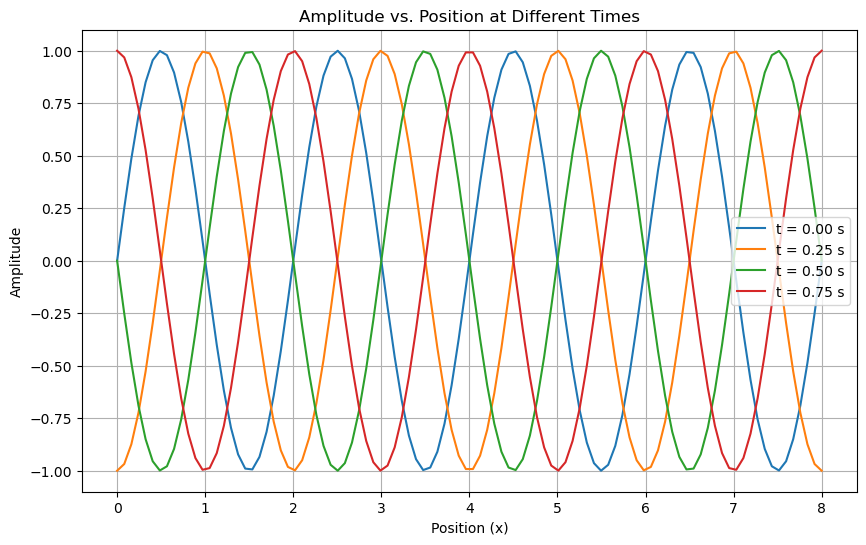
\includegraphics[keepaspectratio,alt={png}]{../images/activity-Waves-1D_activity-Waves-1D_tmp_8_0.png}}
\caption{png}
\end{figure}

\paragraph{Plotting amplitude vs.~time for different
positions}\label{plotting-amplitude-vs.-time-for-different-positions}

At all times the wave is waving, so we can look at the amplitude of the
wave at all times for a single location. We can do this for different
locations.

\begin{Shaded}
\begin{Highlighting}[]
\CommentTok{\# Selected positions to plot}
\NormalTok{positions\_to\_plot }\OperatorTok{=}\NormalTok{ [}\DecValTok{0}\NormalTok{, lambda\_}\OperatorTok{/}\DecValTok{4}\NormalTok{, lambda\_}\OperatorTok{/}\DecValTok{2}\NormalTok{, }\DecValTok{3}\OperatorTok{*}\NormalTok{lambda\_}\OperatorTok{/}\DecValTok{4}\NormalTok{]}

\NormalTok{plt.figure(figsize}\OperatorTok{=}\NormalTok{(}\DecValTok{10}\NormalTok{, }\DecValTok{6}\NormalTok{))}

\ControlFlowTok{for}\NormalTok{ pos }\KeywordTok{in}\NormalTok{ positions\_to\_plot:}
\NormalTok{    plt.plot(t, wave(pos, t), label}\OperatorTok{=}\SpecialStringTok{f\textquotesingle{}x = }\SpecialCharTok{\{}\NormalTok{pos}\SpecialCharTok{:.2f\}}\SpecialStringTok{ units\textquotesingle{}}\NormalTok{)}

\NormalTok{plt.title(}\StringTok{"Amplitude vs. Time at Selected Positions"}\NormalTok{)}
\NormalTok{plt.xlabel(}\StringTok{\textquotesingle{}Time (s)\textquotesingle{}}\NormalTok{)}
\NormalTok{plt.ylabel(}\StringTok{\textquotesingle{}Amplitude\textquotesingle{}}\NormalTok{)}
\NormalTok{plt.legend()}
\NormalTok{plt.grid(}\VariableTok{True}\NormalTok{)}
\NormalTok{plt.show()}
\end{Highlighting}
\end{Shaded}

\begin{figure}
\centering
\pandocbounded{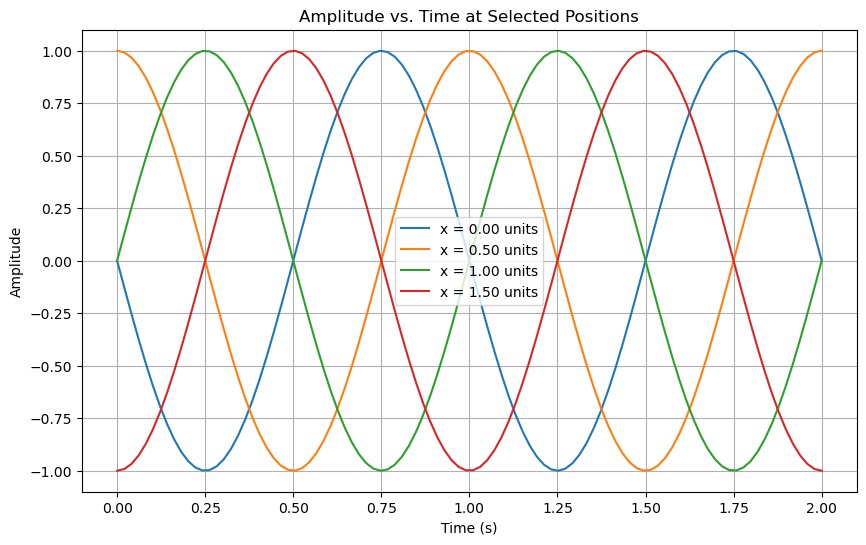
\includegraphics[keepaspectratio,alt={png}]{../images/activity-Waves-1D_activity-Waves-1D_tmp_10_0.png}}
\caption{png}
\end{figure}

\subsubsection{Plotting space and time
together}\label{plotting-space-and-time-together}

It's a bit hard to see what this 1D wave is doing, so we can instead
plot position and time on the plane and let the height represent the
amplitude.

\begin{Shaded}
\begin{Highlighting}[]
\CommentTok{\# Create a 3D plot}
\NormalTok{fig }\OperatorTok{=}\NormalTok{ plt.figure(figsize}\OperatorTok{=}\NormalTok{(}\DecValTok{12}\NormalTok{, }\DecValTok{8}\NormalTok{))}
\NormalTok{ax }\OperatorTok{=}\NormalTok{ fig.add\_subplot(}\DecValTok{111}\NormalTok{, projection}\OperatorTok{=}\StringTok{\textquotesingle{}3d\textquotesingle{}}\NormalTok{)}

\NormalTok{ax.plot\_surface(X, T, Y, cmap}\OperatorTok{=}\StringTok{\textquotesingle{}inferno\textquotesingle{}}\NormalTok{)  }\CommentTok{\# Using viridis colormap for better clarity}
\NormalTok{ax.set\_title(}\StringTok{"3D Plot of Traveling Wave in Space and Time"}\NormalTok{)}
\NormalTok{ax.set\_xlabel(}\StringTok{"Position (x)"}\NormalTok{)}
\NormalTok{ax.set\_ylabel(}\StringTok{"Time (t)"}\NormalTok{)}
\NormalTok{ax.set\_zlabel(}\StringTok{"Amplitude"}\NormalTok{)}
\NormalTok{ax.view\_init(elev}\OperatorTok{=}\DecValTok{30}\NormalTok{, azim}\OperatorTok{={-}}\DecValTok{60}\NormalTok{)  }\CommentTok{\# Adjust viewing angle for better visualization}
\end{Highlighting}
\end{Shaded}

\begin{figure}
\centering
\pandocbounded{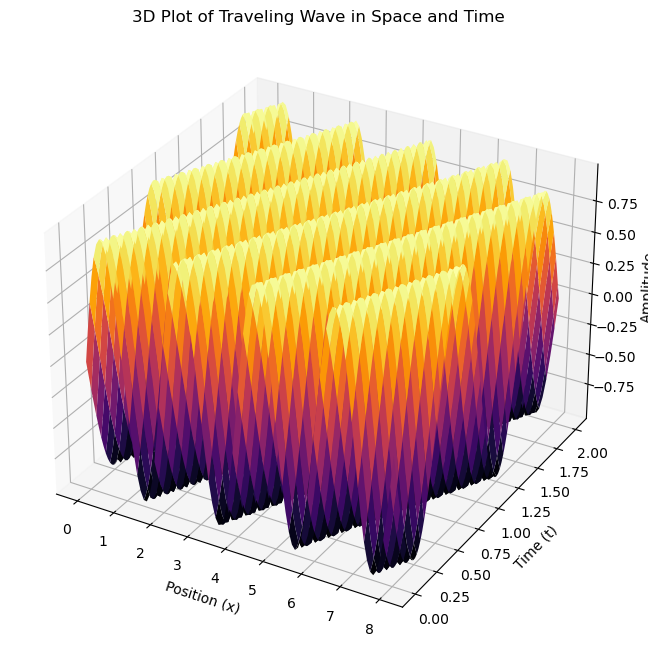
\includegraphics[keepaspectratio,alt={png}]{../images/activity-Waves-1D_activity-Waves-1D_tmp_12_0.png}}
\caption{png}
\end{figure}

\paragraph{Ok, but make it 2D.}\label{ok-but-make-it-2d.}

This isn't the easiest representation to view. You might be able to
adjust it a bit with changing the viewing angle. But, we can flatten
this plot into a heat map. This is the more common way of viewing these
kind of data.

\begin{Shaded}
\begin{Highlighting}[]
\NormalTok{plt.figure(figsize}\OperatorTok{=}\NormalTok{(}\DecValTok{10}\NormalTok{, }\DecValTok{6}\NormalTok{))}
\NormalTok{plt.imshow(Y, aspect}\OperatorTok{=}\StringTok{\textquotesingle{}auto\textquotesingle{}}\NormalTok{, origin}\OperatorTok{=}\StringTok{\textquotesingle{}lower\textquotesingle{}}\NormalTok{, extent}\OperatorTok{=}\NormalTok{[x.}\BuiltInTok{min}\NormalTok{(), x.}\BuiltInTok{max}\NormalTok{(), t.}\BuiltInTok{min}\NormalTok{(), t.}\BuiltInTok{max}\NormalTok{()], cmap}\OperatorTok{=}\StringTok{\textquotesingle{}inferno\textquotesingle{}}\NormalTok{)}
\NormalTok{plt.colorbar(label}\OperatorTok{=}\StringTok{"Amplitude"}\NormalTok{)}
\NormalTok{plt.title(}\StringTok{"2D Heatmap of Traveling Wave in Space and Time"}\NormalTok{)}
\NormalTok{plt.xlabel(}\StringTok{"Position (x)"}\NormalTok{)}
\NormalTok{plt.ylabel(}\StringTok{"Time (t)"}\NormalTok{)}

\NormalTok{plt.show()}
\end{Highlighting}
\end{Shaded}

\begin{figure}
\centering
\pandocbounded{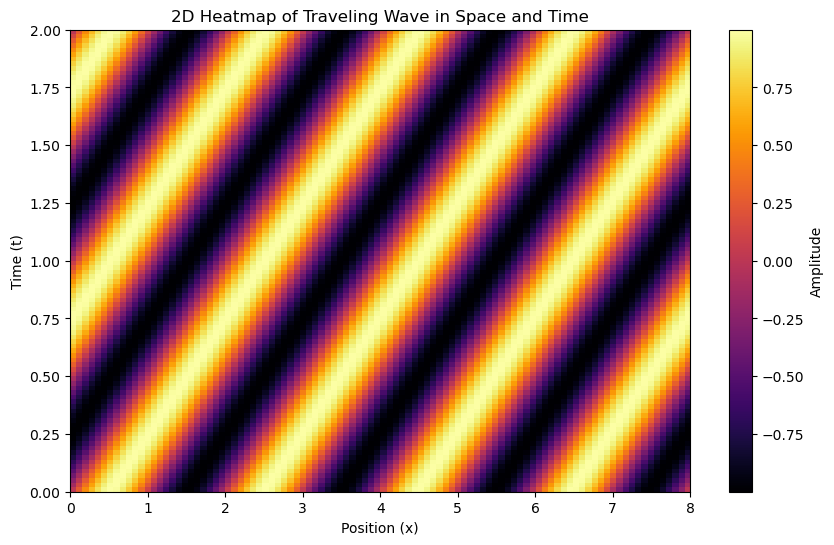
\includegraphics[keepaspectratio,alt={png}]{../images/activity-Waves-1D_activity-Waves-1D_tmp_14_0.png}}
\caption{png}
\end{figure}

\paragraph{But I really want to animate
it}\label{but-i-really-want-to-animate-it}

Sure. Here's that code.

\begin{Shaded}
\begin{Highlighting}[]
\NormalTok{fig, ax }\OperatorTok{=}\NormalTok{ plt.subplots(figsize}\OperatorTok{=}\NormalTok{(}\DecValTok{10}\NormalTok{, }\DecValTok{6}\NormalTok{))}
\NormalTok{line, }\OperatorTok{=}\NormalTok{ ax.plot(x, wave(x, }\DecValTok{0}\NormalTok{))  }\CommentTok{\# Initial plot (t=0)}
\NormalTok{ax.set\_ylim([}\OperatorTok{{-}}\NormalTok{A, A])  }\CommentTok{\# Setting the y limits to the amplitude range}
\NormalTok{ax.set\_xlabel(}\StringTok{\textquotesingle{}Position (x)\textquotesingle{}}\NormalTok{)}
\NormalTok{ax.set\_ylabel(}\StringTok{\textquotesingle{}Amplitude\textquotesingle{}}\NormalTok{)}
\NormalTok{ax.grid(}\VariableTok{True}\NormalTok{)}
\NormalTok{ax.set\_title(}\StringTok{"Amplitude vs. Position over Time"}\NormalTok{)}

\KeywordTok{def}\NormalTok{ update(frame):}
\NormalTok{    line.set\_ydata(wave(x, frame))  }\CommentTok{\# Update the y data of the line plot for the current time frame}
\NormalTok{    ax.set\_title(}\SpecialStringTok{f"Amplitude vs. Position at t = }\SpecialCharTok{\{}\NormalTok{frame}\SpecialCharTok{:.2f\}}\SpecialStringTok{ s"}\NormalTok{)}
    \ControlFlowTok{return}\NormalTok{ line,}

\CommentTok{\# Animate over the given times using FuncAnimation}
\NormalTok{ani }\OperatorTok{=}\NormalTok{ FuncAnimation(fig, update, frames}\OperatorTok{=}\NormalTok{t, blit}\OperatorTok{=}\VariableTok{True}\NormalTok{, interval}\OperatorTok{=}\DecValTok{50}\NormalTok{)}
\NormalTok{plt.close(fig) }\CommentTok{\#\# needed to stop another static image from being displayed}

\CommentTok{\# Display the animation in the notebook}
\NormalTok{HTML(ani.to\_jshtml())}
\end{Highlighting}
\end{Shaded}

\begin{verbatim}
<input id="_anim_slider3a4ba7a62c13475c8b9940f195fcfc0e" type="range" class="anim-slider"
       name="points" min="0" max="1" step="1" value="0"
       oninput="anim3a4ba7a62c13475c8b9940f195fcfc0e.set_frame(parseInt(this.value));">
<div class="anim-buttons">
  <button title="Decrease speed" aria-label="Decrease speed" onclick="anim3a4ba7a62c13475c8b9940f195fcfc0e.slower()">
      <i class="fa fa-minus"></i></button>
  <button title="First frame" aria-label="First frame" onclick="anim3a4ba7a62c13475c8b9940f195fcfc0e.first_frame()">
    <i class="fa fa-fast-backward"></i></button>
  <button title="Previous frame" aria-label="Previous frame" onclick="anim3a4ba7a62c13475c8b9940f195fcfc0e.previous_frame()">
      <i class="fa fa-step-backward"></i></button>
  <button title="Play backwards" aria-label="Play backwards" onclick="anim3a4ba7a62c13475c8b9940f195fcfc0e.reverse_animation()">
      <i class="fa fa-play fa-flip-horizontal"></i></button>
  <button title="Pause" aria-label="Pause" onclick="anim3a4ba7a62c13475c8b9940f195fcfc0e.pause_animation()">
      <i class="fa fa-pause"></i></button>
  <button title="Play" aria-label="Play" onclick="anim3a4ba7a62c13475c8b9940f195fcfc0e.play_animation()">
      <i class="fa fa-play"></i></button>
  <button title="Next frame" aria-label="Next frame" onclick="anim3a4ba7a62c13475c8b9940f195fcfc0e.next_frame()">
      <i class="fa fa-step-forward"></i></button>
  <button title="Last frame" aria-label="Last frame" onclick="anim3a4ba7a62c13475c8b9940f195fcfc0e.last_frame()">
      <i class="fa fa-fast-forward"></i></button>
  <button title="Increase speed" aria-label="Increase speed" onclick="anim3a4ba7a62c13475c8b9940f195fcfc0e.faster()">
      <i class="fa fa-plus"></i></button>
</div>
<form title="Repetition mode" aria-label="Repetition mode" action="#n" name="_anim_loop_select3a4ba7a62c13475c8b9940f195fcfc0e"
      class="anim-state">
  <input type="radio" name="state" value="once" id="_anim_radio1_3a4ba7a62c13475c8b9940f195fcfc0e"
         >
  <label for="_anim_radio1_3a4ba7a62c13475c8b9940f195fcfc0e">Once</label>
  <input type="radio" name="state" value="loop" id="_anim_radio2_3a4ba7a62c13475c8b9940f195fcfc0e"
         checked>
  <label for="_anim_radio2_3a4ba7a62c13475c8b9940f195fcfc0e">Loop</label>
  <input type="radio" name="state" value="reflect" id="_anim_radio3_3a4ba7a62c13475c8b9940f195fcfc0e"
         >
  <label for="_anim_radio3_3a4ba7a62c13475c8b9940f195fcfc0e">Reflect</label>
</form>
\end{verbatim}

\begin{Shaded}
\begin{Highlighting}[]
\CommentTok{\#\# your code here}

\CommentTok{\#\# REMEMBER THAT YOU ARE WORKING ON SUPERPOSITION OF WAVES}
\end{Highlighting}
\end{Shaded}

\subsection{Implications of Superposition:
Diffraction}\label{implications-of-superposition-diffraction}

One of the key indicators of wave like behavior is
\href{https://en.wikipedia.org/wiki/Diffraction}{diffraction}.
Diffraction is the bending of waves around obstacles and it is a
consequence of superposition.

In the case of
\href{https://en.wikipedia.org/wiki/Diffraction\#Single-slit_diffraction}{single-slit
diffraction}, the wave is diffracted around a slit of width \(a\). a
forms circular wave fronts that interfere with each other.

\begin{figure}
\centering
\pandocbounded{\includegraphics[keepaspectratio,alt={Diagram of single slit diffraction}]{../images/activity-Waves-1D_Single_slit_diffraction.jpeg}}
\caption{Diagram of single slit diffraction}
\end{figure}

A screen placed a distance \(L\) away from the slit will show a
diffraction pattern. We can show the intensity of the diffraction
pattern is:

\[I(\theta) = I_0\left(\dfrac{\sin(\beta)}{\beta}\right)^2\]

where

\[\beta = \dfrac{\pi a \sin(\theta)}{\lambda}\]

and \(\lambda\) is the wavelength of the wave and \(\theta\) is the
angle of the diffracted wave from the center of the slit
(\(\tan(\theta) = y/L\) where \(y\) is the location along the screen).

\textbf{✅ Do this}

\begin{enumerate}
\def\labelenumi{\arabic{enumi}.}
\tightlist
\item
  Plot the intensity of the diffraction pattern for a single slit of
  width \(a=1\) mm and wavelength \(\lambda=500\) nm.
\item
  Find the slit width needed to form a diffraction pattern for a typical
  water wave. You will need to make some estimates.
\item
  For atomic spacing (\(10^{-10}\) m), use your plotting tool to
  estimate the wavelength needed to form a diffraction pattern. You will
  need to make some estimates.
\end{enumerate}

\begin{Shaded}
\begin{Highlighting}[]
\CommentTok{\#\# your code here}
\end{Highlighting}
\end{Shaded}

\begin{Shaded}
\begin{Highlighting}[]

\end{Highlighting}
\end{Shaded}
